%!TEX root = ../my_thesis.tex

\appendix

\chapter{Compléments au Chapitre 1}

\section{Détails des calculs de l'algorithme APP}\label{append:app}
Cette partie vise à démontrer l'ensemble des calculs présentés dans la section \ref{sec:BCJR}.
\subsection{Décomposition de la probabilité jointe} 
Cette décomposition est basée sur le partitionnement de la séquence reçue $\mathbf{y}$ en trois sous-séquences. La première représentant le passé $ \mathbf{y_{<k}}$, la seconde le présent $\mathbf{y_{k}} $ et enfin le futur $ \mathbf{y_{>k}}$.

Le calcul suivant est basé sur la relation de Bayes : $P(A|B) = \frac{P(A,B)}{P(B)}$ et sa version ternaire $P(A|B,C) = \frac{P(A,B|C)}{P(B|C)}$.

Aussi, sont nécessaires au déroulement de ce calcul les propriétés de Markov du treillis de l'encodeur RSC considéré. En effet :
\begin{align*}
	\hspace*{-4ex}
	P(s_{k-1}=s, s_{k}=s',\mathbf{y}) & = P(s_{k-1}=s, s_{k}=s',\mathbf{y_{<k}},\mathbf{y_{k}},\mathbf{y_{>k}})                                                                                                                             \\
	                                  & = P(\mathbf{y_{>k}}|s_{k-1}=s, s_{k}=s',\mathbf{y_{<k}},\mathbf{y_{k}})\times P(s_{k-1}=s, s_{k}=s',\mathbf{y_{<k}},\mathbf{y_{k}})                                                                 \\
	                                  & =P(\mathbf{y_{>k}}|s_{k}=s')\times P(s_{k-1}=s, s_{k}=s',\mathbf{y_{<k}},\mathbf{y_{k}})                                                                                                            \\
	                                  & =P(\mathbf{y_{>k}}|s_{k}=s')\times P(s_{k}=s',\mathbf{y_{k}}|s_{k-1}=s,\mathbf{y_{<k}})\times P(s_{k-1}=s,\mathbf{y_{<k}})                                                                          \\
	                                  & = \underbrace{P(\mathbf{y_{>k}}|s_{k}=s')}_{\beta_k(s')}\times \underbrace{P(s_{k}=s',\mathbf{y_{k}}|s_{k-1}=s)}_{\gamma_k(s,s')}\times \underbrace{P(s_{k-1}=s,\mathbf{y_{<k}})}_{\alpha_{k-1}(s)} \\
	                                  & = \alpha_{k-1}(s) \times \gamma_k(s,s') \times \beta_k(s')                                                                                                                                          
\end{align*}

\subsection{Calcul récursif de $\alpha$}
Par définition, $\alpha_{k-1}(s) = P(s_{k-1}=s,\mathbf{y_{<k}})$. Or, sachant que $\sum\limits_B P(A,B) = P(A)$ et en appliquant le théorème de Bayes,
\begin{align*}
	\hspace*{-4ex}
	\alpha_k(s) & = \sum\limits_{s'}P(s_{k}=s,s_{k-1}=s',\mathbf{y_{<k}},\mathbf{y_k})                                        \\
	            & = \sum\limits_{s'}P(s_{k}=s,\mathbf{y_k} | s_{k-1}=s',\mathbf{y_{<k}}) \times P(s_{k-1}=s',\mathbf{y_{<k}}) \\
	            & = \sum\limits_{s'}P(s_{k}=s,\mathbf{y_k} | s_{k-1}=s') \times P(s_{k-1}=s',\mathbf{y_{<k}})                 \\
	            & = \sum\limits_{s'}\gamma_k(s',s)\times \alpha_{k-1}(s')                                                     
\end{align*}
Ainsi, les valeurs de $\alpha_k(s)$ peuvent être calculées récursivement en parcourant le treillis dans l'ordre chronologique, à partir des valeurs initiales $\alpha_0(s)$ et des probabilités de transition.

\subsection{Calcul récursif de $\beta$}
En utilisant les mêmes propriétés calculatoires que pour le calcul de $\alpha$ : 
\begin{align*}
	\hspace*{-4ex}
	\beta_{k-1}(s) & = P(\mathbf{y_{>k-1}}|s)                                                             \\
	               & = \sum\limits_{s'}P(s',\mathbf{y_{k}},\mathbf{y_{>k}|s})                             \\
	               & = \sum\limits_{s'}P(\mathbf{y_{>k}} | s',s, \mathbf{y_{k}}) P(s', \mathbf{y_{k}}| s) \\
	               & = \sum\limits_{s'}P(\mathbf{y_{>k}} | s') P(s', \mathbf{y_{k}}| s)                   \\
	               & = \sum\limits_{s'}\gamma_k(s,s')\times \beta_{k}(s')                                 
\end{align*}


\subsection{Calcul de la probabilité \textit{a posteriori}}
La probabilité \textit{a posteriori} a pour expression : 
\begin{align*}
	\|\mathbf{y}_k-\mathbf{c}_k\|^2 & = (y_k^s - c_k^s)^2 + (y_k^p - c_k^p)^2                                               \\
	                                & = (y_k^s)^2 - 2  y_k^s   c_k^s +  (c_k^s)^2 + (y_k^p)^2 - 2  y_k^p c_k^p +  (c_k^p)^2 \\
	                                & = (y_k^s)^2 +   (y_k^p)^2 + 2  - 2*( y_k^s   c_k^s +  y_k^p c_k^p)                    
\end{align*}

Ainsi, \[\gamma_k(s,s') = \frac{P(m_k)}{2\pi\sigma^2}\exp\left(-\frac{ (y_k^s)^2 +   (y_k^p)^2 + 2}{2\sigma^2}\right) \exp\left(\frac{( y_k^s   c_k^s +  y_k^p c_k^p)}{\sigma^2}\right)\]

Or, la première exponentielle n'est pas dépendante de $m_k$ (ou du chemin $ s \mapsto s'$) et peut donc être supprimé du numérateur et du dénominateur dans l’expression de la probabilité \textit{a posteriori}.


\section{Détails des calculs pour les algorithmes sub-APP}\label{append:subAPP}
\subsection{Calcul des métriques}
Dans le cadre des algorithmes sub-APP, les probabilités manipulées sont transformées en métriques en prenant le logarithme népérien de celles-ci. Ainsi, nous avons :
\begin{align*}
	\tilde{\alpha}_k(s) & = \ln \sum\limits_{s'}\alpha_{k-1}(s')\times\gamma_k(s',s)                                                     \\
	                    & = \ln \sum\limits_{s'} \exp\left(\tilde{\alpha}_{k-1}(s')\right)\times\exp\left(\tilde{\gamma}_k(s', s)\right) \\
	                    & = \ln \sum\limits_{s'} \exp\left(\tilde{\alpha}_{k-1}(s') + \tilde{\gamma}_k(s', s)\right)                     
\end{align*}
Des calculs très similaires permettent d'obtenir $\tilde{\beta}_k(s)$ et $\tilde{\gamma}_k(s,s')$.

\subsection{Opérateur $\maxstar$}\label{append:maxstar}
En partant de la définition de l’opérateur $\maxstar$ et en utilisant une disjonction de cas, on obtient : 
\begin{align*}
	\maxstar(x,y) & = \ln\left(\e^x+\e^y\right)              \\
	              & =\begin{cases}                           
	\ln	\left(\e^x\left(1+\e^{y-x}\right)\right) \text{si} x>y  \\
	\ln	\left(\e^y\left(1+\e^{x-y}\right)\right) \text{si} x<y
	\end{cases}\\
	              & =\begin{cases}                           
	x + \ln\left(1+\e^{y-x}\right) \quad\text{si}\quad x>y  \\
	y+\ln\left(1+\e^{x-y}\right) \quad\text{si}\quad x<y
	\end{cases}\\
	              & =\max(x,y) +\ln\left(1+\e^{|x-y|}\right) 
\end{align*}


% Ainsi, en reprenant les définitions récursives et en substituant les probabilités par les métriques, leurs expressions deviennent : 
% \begin{align*}
% 	M^\alpha_k(s) & = \ln \sum\limits_{s'}\alpha_{k-1}(s')\times\gamma_k(s',s)                                         \\
% 	              & = \ln \sum\limits_{s'} \exp\left(M^\alpha_{k-1}(s')\right)\times\exp\left(M^\gamma_k(s', s)\right) \\
% 	              & = \ln \sum\limits_{s'} \exp\left(M^\alpha_{k-1}(s') + M^\gamma_k(s', s)\right)                     
% \end{align*}
% et 
% \[M^\beta_k(s) = \ln \sum\limits_{s'} \exp\left(M^\beta_{k+1}(s') + M^\gamma_{k+1}(s, s')\right)\]
% avec pour conditions initiales, 

% De même les LLR \textit{a posteriori} deviennent :
% \begin{align*} 
% 	L(m_k) & = \ln \sum\limits_{s,s'\in S_1} \exp\left( M^\alpha_{k-1}(s) + M^\gamma_{k}(s, s') + M^\beta_k(s') \right)       \\ 
% 	       & \quad - \ln \sum\limits_{s,s'\in S_0} \exp\left( M^\alpha_{k-1}(s) + M^\gamma_{k}(s, s') + M^\beta_k(s') \right) 
% \end{align*}
% Toutefois, ces réécritures dans le domaines logarithmiques ne permettent pas encore de réduire la complexité calculatoire. Pour ce faire, introduisons l'opérateur \[\maxstar(x,y) = \ln(\mathrm{e}^x + \mathrm{e}^y).\]
% Ainsi, les métriques précédentes deviennent : 



% Il est démontré facilement (en utilisant un disjonction de cas) que :
% \[\maxstar(x,y) = \max(x,y) + \ln(1+e^{|x-y|})\]
% \paragraph{Stabilité numérique}


\chapter{Compléments au Chapitre 2}
\section{Standard CCSDS}\label{sec:annCCSDS}
Cette section présente les observations statistiques obtenues avec le standard CCSDS. La Figure \ref{fig:m_ccsds} présente 
les valeurs moyennes d'oscillations, ce pour différentes valeurs de SNR. Les Figures \ref{fig:it1_ccsds} et \ref{fig:it2_ccsds}
présentent l'évolution des oscillations au cours des itérations pour, respectivement, un taux d'erreur trame correspondant 
au seuil de convergence et un correspondant au plancher d'erreur. Finalement, les Figures \ref{fig:d1_ccsds} et \ref{fig:d2_ccsds} 
présentent la distribution normalisée des oscillations pour ces deux valeurs de SNR considérées.
\begin{figure}[tb]
	\begin{center}
	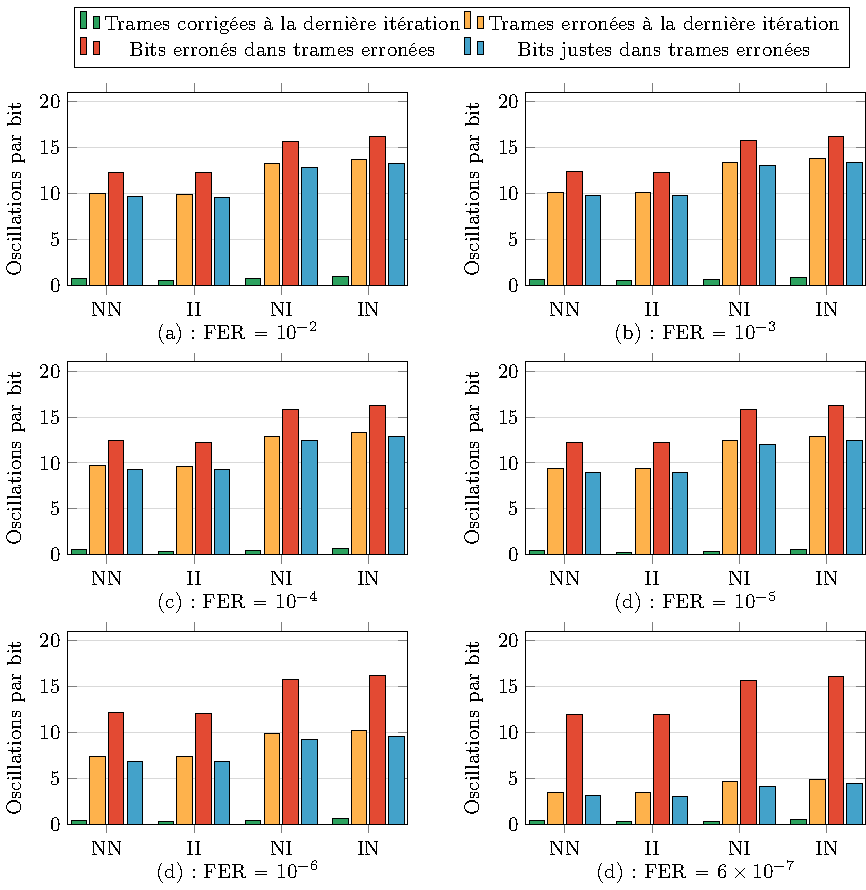
\includegraphics[width=.9\textwidth]{main/ch2_fig/tikz/m_ccsds.pdf}
	\caption{Nombre moyen d'oscillations pour différents taux d'erreurs trame cibles, turbo code du standard CCSDS (K=1784, R=1/3) \label{fig:m_ccsds}}
	\end{center}
\end{figure}

\begin{figure}[!ht]
	%\hspace*{-.7cm}	
	\begin{center}
	\includegraphics[width=.9\textwidth]{main/ch2_fig/tikz/it_ccsds10-2.pdf}
	\caption{Oscillations au cours des itérations dans le cadre du standard CCSDS (K=1784, R=1/3) pour un taux d'erreur trame de $10^{-2}$\label{fig:it1_ccsds}}
	\end{center}
\end{figure}

\begin{figure}[!ht]
	%\hspace*{-.7cm}
	\begin{center}
	\includegraphics[width=.9\textwidth]{main/ch2_fig/tikz/it_ccsds610-7.pdf}
	\caption{Oscillations au cours des itérations dans le cadre du standard CCSDS (K=1784, R=1/3) pour un taux d'erreur trame de $6\times10^{-7}$\label{fig:it2_ccsds}}
	\end{center}
\end{figure}

\begin{figure}[!ht]
	\centering
	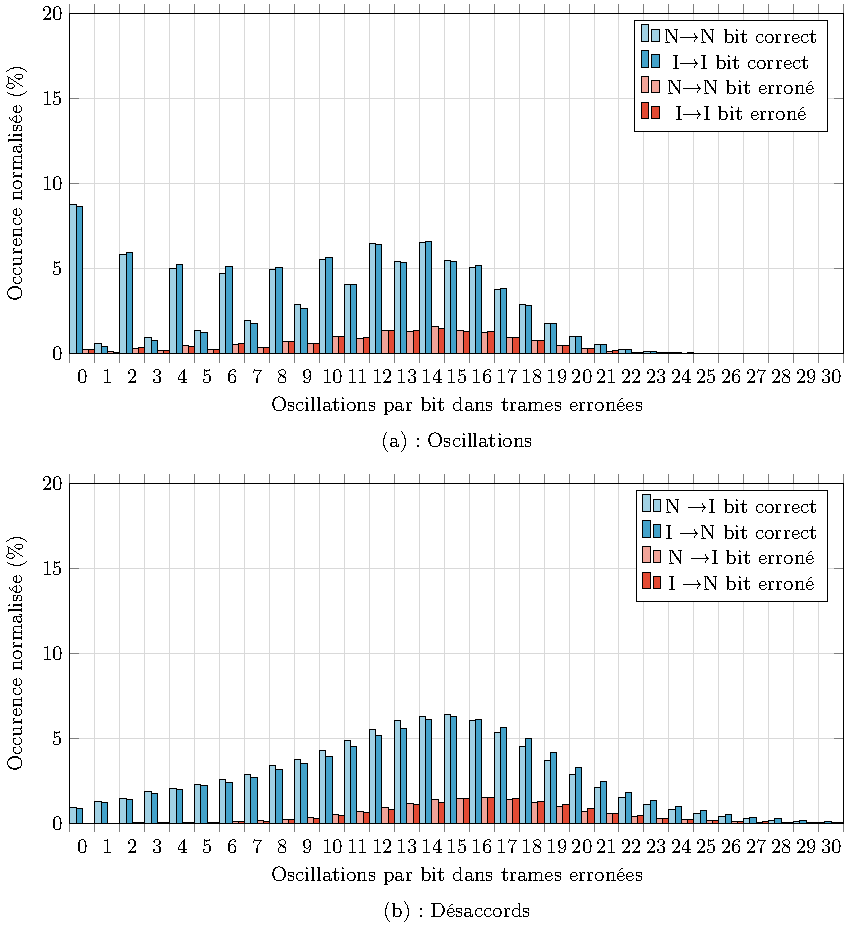
\includegraphics[width=.9\textwidth]{main/ch2_fig/tikz/d_ccsds_10-2.pdf}
	\caption{Distribution du nombre d'oscillations par bit pour un taux d'erreur trame de $10^{-2}$, pour le turbo code du standard CCSDS (K=1784, R=1/3)\label{fig:d1_ccsds}}
\end{figure}

\begin{figure}[!ht]
	\centering
	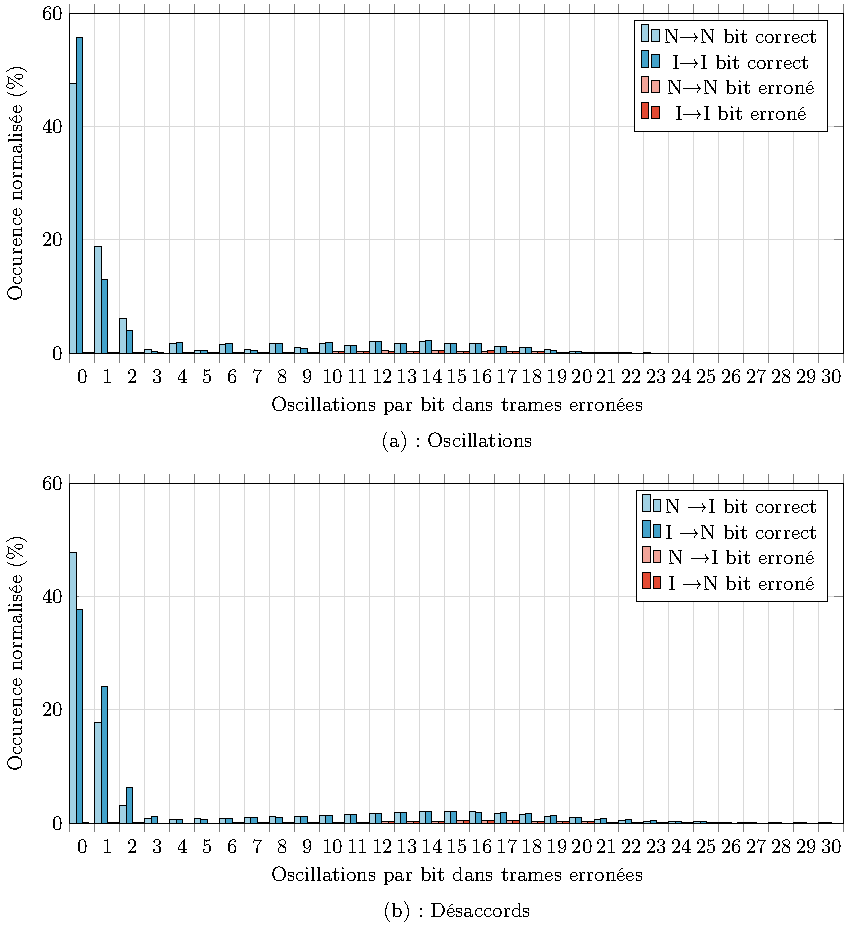
\includegraphics[width=.9\textwidth]{main/ch2_fig/tikz/d_ccsds_610-7.pdf}
	\caption{Distribution du nombre d'oscillations par bit pour un taux d'erreur trame de $6\times10^{-7}$, pour le turbo code du standard CCSDS (K=1784, R=1/3)\label{fig:d2_ccsds}}
\end{figure}


\chapter{Compléments au Chapitre 3}\label{sec:ann3}
\newpage
\begin{adjustbox}{angle=90, caption={Spectres de distances de turbo codes binaires standardisés},float=table}
\centering
\resizebox{1.5\textwidth}{!}{
\begin{tabular}{@{}llrrrrrrrrrrrrrrrrrrrrrrrrrrrr@{}}
\toprule
\multirow{15}{*}{\textbf{LTE}} & \multirow{3}{*}{\textbf{K=528}}  & \textbf{d} & 23 & 24 & 25 & 26 & 27 & 28 & 29 & 30 & 31 & 32 & 33 & 34 & 35 & 36 & 37   & 38   & 39    & 40   & 41  & 42  & 43   & 44   & 45   & 46  & 47   & 48  & 49  \\  
                    &    & \textbf{a} & 1  & 1  & 1  & 0  & 3  & 3  & 6  & 0  & 6  & 4  & 11 & 10 & 14 & 12 & 96   & 886  & 1421  & 45   & 123 & 156 & 192  & 227  & 140  & 55  & 285  & 52  & 62  \\
                    &    & \textbf{w} & 1  & 2  & 3  & 0  & 9  & 6  & 16 & 0  & 20 & 16 & 39 & 32 & 58 & 50 & 318  & 5268 & 12535 & 210  & 779 & 864 & 984  & 982  & 850  & 286 & 1415 & 260 & 292 \\ \cdashlinelr{2-30}
& \multirow{3}{*}{\textbf{K=1024}} & \textbf{d} & 27 & 28 & 29 & 30 & 31 & 32 & 33 & 34 & 35 & 36 & 37 & 38 & 39 & 40 & 41   & 42   & 43    & 44   & 45  & 46  & 47   & 48   & 49   &     &      &     &     \\
  &                      & \textbf{a} & 1  & 2  & 3  & 1  & 2  & 1  & 2  & 2  & 7  & 3  & 7  & 9  & 11 & 11 & 20   & 30   & 147   & 437  & 49  & 64  & 583  & 179  & 511  &     &      &     &     \\
   &                     & \textbf{w} & 1  & 4  & 9  & 2  & 6  & 2  & 6  & 6  & 21 & 12 & 27 & 32 & 43 & 44 & 78   & 142  & 719   & 1770 & 241 & 326 & 2949 & 1148 & 3407 &     &      &     &     \\ \cdashlinelr{2-30}
& \multirow{3}{*}{\textbf{K=1504}} & \textbf{d} & 25 & 26 & 27 & 28 & 29 & 30 & 31 & 32 & 33 & 34 & 35 & 36 & 37 & 38 & 39   & 40   & 41    & 42   & 43  & 44  & 45   & 46   & 47   & 48  & 49   &     &     \\
  &                      & \textbf{a} & 1  & 0  & 0  & 1  & 1  & 1  & 2  & 1  & 2  & 5  & 1  & 6  & 7  & 3  & 14   & 13   & 17    & 22   & 32  & 28  & 47   & 49   & 185  & 91  & 1414 &     &     \\
   &                     & \textbf{w} & 3  & 0  & 0  & 2  & 3  & 2  & 6  & 4  & 6  & 18 & 3  & 22 & 23 & 12 & 54   & 54   & 75    & 90   & 154 & 126 & 223  & 246  & 909  & 486 & 9696 &     &     \\ \cdashlinelr{2-30}
& \multirow{3}{*}{\textbf{K=2048}} & \textbf{d} & 27 & 28 & 29 & 30 & 31 & 32 & 33 & 34 & 35 & 36 & 37 & 38 & 39 & 40 & 41   & 42   & 43    & 44   & 45  & 46  & 47   & 48   & 49   &     &      &     &     \\
  &                      & \textbf{a} & 1  & 2  & 1  & 0  & 3  & 0  & 2  & 1  & 2  & 1  & 1  & 3  & 8  & 5  & 12   & 15   & 16    & 425  & 23  & 37  & 240  & 45   & 290  &     &      &     &     \\
   &                     & \textbf{w} & 1  & 4  & 3  & 0  & 9  & 0  & 6  & 4  & 6  & 4  & 3  & 8  & 26 & 20 & 44   & 62   & 72    & 1702 & 117 & 178 & 1180 & 230  & 1872 &     &      &     &     \\ \cdashlinelr{2-30}
& \multirow{3}{*}{\textbf{K=6144}} & \textbf{d} & 26 & 27 & 28 & 29 & 30 & 31 & 32 & 33 & 34 & 35 & 36 & 37 & 38 & 39 & 40   & 41   & 42    & 43   & 44  & 45  & 46   & 47   & 48   & 49  &      &     &     \\
  &                      & \textbf{a} & 1  & 0  & 0  & 0  & 0  & 0  & 1  & 1  & 1  & 0  & 1  & 1  & 1  & 2  & 3    & 7    & 9     & 10   & 6   & 8   & 10   & 21   & 20   & 25  &      &     &     \\
   &                     & \textbf{w} & 2  & 0  & 0  & 0  & 0  & 0  & 4  & 3  & 4  & 0  & 4  & 3  & 4  & 8  & 12   & 25   & 34    & 46   & 30  & 40  & 42   & 99   & 102  & 135 &      &     &     \\ \cdashlinelr{1-30}
\multirow{3}{*}{\textbf{\textbf{CCSDS}}} & \multirow{3}{*}{\textbf{K=1784}} & \textbf{d} & 34 & 35 & 36 & 37 & 38 & 39 & 40 & 41 & 42 & 43 & 44 & 45 & 46 & 47 & 48   & 49   &       &      &     &     &      &      &      &     &      &     &     \\
    &                    & \textbf{a} & 1  & 0  & 0  & 7  & 4  & 2  & 5  & 2  & 5  & 4  & 3  & 6  & 7  & 4  & 713  & 8    &       &      &     &     &      &      &      &     &      &     &     \\
     &                   & \textbf{w} & 2  & 0  & 0  & 17 & 9  & 6  & 13 & 5  & 14 & 18 & 6  & 19 & 39 & 21 & 4248 & 39   &       &      &     &     &      &      &      &     &      &     &     \\ \bottomrule
\end{tabular}}
\end{adjustbox}

\newpage
\begin{adjustbox}{angle=90, caption={Spectres de distance de turbo codes du standard DVB-RCS},float=table}
\centering
\resizebox{1.5\textwidth}{!}{
\begin{tabular}{@{}llrrrrrrrrrrrrrrrrrrrrrrrrrrrr@{}}
\toprule
\multirow{16}{*}{\textbf{K=440}} 
& \multirow{4}{*}{\textbf{R=1/2}}  & \textbf{d}  &   16&   17&   18&   19&   20&   21&   22&   23&   24&   25&   26&   27&   28&   29&   30&   31&   32&   33&   34&   35&   36&   37&   38&   39&   40 \\
&                                  & \textbf{a}  &  110&    0&  220&    0&  440&  220&  770& 1962&  998& 2006& 1279&  942&  475&  379&  135&   32&  307&   31&  195&   12&  388&  207&  138&   54&   11 \\
&                                  & \textbf{w}  & 1100&    0& 1870&    0& 3740& 1980& 5610&19616& 8881&17439&11145& 7182& 3530& 2679& 1458&  313& 1944&  278& 1348&   89& 2964& 1677&  858&  485&  107 \\
&                                  & \textbf{ws} &  770&    0& 1320&    0& 2750& 1540& 4510&13533& 6216&12215& 7718& 5120& 2721& 1935& 1015&  213& 1392&  201&  954&   63& 2205& 1254&  648&  294&   78 \\
\cdashlinelr{2-30}
& \multirow{4}{*}{\textbf{R=1/3}}  & \textbf{d}  &   28&   29&   30&   31&   32&   33&   34&   35&   36&   37&   38&   39&   40&   41&   42&   43&   44&   45&   46&   47&   48&   49&   50&   51&   52 \\
&                                  & \textbf{a}  &  110&    0&  220&    0&    0&    0&  220&  110& 1209&  868&  329&  532& 1307& 1069&  976& 1025&  642&  653&  454&  231&  267&   34&  115&   14&   20 \\
&                                  & \textbf{w}  & 1100&    0& 1870&    0&    0&    0& 2200& 1210& 9889& 7690& 3181& 5926&10702& 9020& 8509& 8231& 6470& 5746& 4098& 1747& 2367&  284& 1349&   87&  170 \\
&                                  & \textbf{ws} &  770&    0& 1320&    0&    0&    0& 1540&  880& 7472& 5636& 2523& 4099& 7855& 6548& 5884& 6276& 4263& 4154& 2512& 1170& 1661&  202&  905&   73&  125 \\
\cdashlinelr{2-30}
& \multirow{4}{*}{\textbf{R=3/4}} & \textbf{d}  &     8&    9&   10&   11&   12&   13&   14&   15&   16&   17&   18&   19&   20&   21&   22&   23&   24&   25&   26&   27&   28&   29&   30&   31&   32 \\
&                                 & \textbf{a}  &    27&  193&  600& 2319& 5490& 3348&  918&  756&  668&  627&  582&  673&  612&  771&  785&  813&  849&  851&  882&  791&  804&  665&  752&  624&  632 \\
&                                 & \textbf{w}  &   108&  810& 3439&13675&34710&20506& 5601& 4748& 4264& 4046& 3672& 4232& 3840& 4855& 5077& 5175& 5508& 5561& 5783& 4966& 4928& 4433& 4625& 3993& 4182 \\
&                                 & \textbf{ws} &   108&  741& 2939&11424&28458&16658& 4581& 3873& 3519& 3293& 2990& 3443& 3138& 3933& 4122& 4135& 4475& 4484& 4636& 4053& 4087& 3672& 3730& 3299& 3416 \\
\cdashlinelr{2-30}
& \multirow{4}{*}{\textbf{R=6/7}} & \textbf{d}  &     4&    5&    6&    7&    8&    9&   10&   11&   12&   13&   14&   15&   16&   17&   18&   19&   20&   21&   22&   23&   24&   25&   26&   27&   28 \\
&                                 & \textbf{a}  &    10&   51&  615& 3376& 8394& 1915& 1382& 1429& 1266& 1406& 1416& 1419& 1448& 1317& 1361& 1504& 1474& 1513& 1666& 1632& 1722& 1601& 1632& 1652& 1888 \\
&                                 & \textbf{w}  &    40&  206& 2810&16954&47379&10556& 7800& 8037& 7274& 8193& 7964& 7960& 8046& 7520& 7864& 8425& 8541& 8517& 9422& 9322& 9698& 8937& 9149& 9231&10589 \\
&                                 & \textbf{ws} &    40&  193& 2681&15833&43467& 9577& 7140& 7315& 6672& 7450& 7297& 7242& 7375& 6855& 7244& 7801& 7852& 7873& 8725& 8666& 8974& 8210& 8424& 8538& 9800 \\
\toprule
\multirow{12}{*}{\textbf{K=752}}
& \multirow{4}{*}{\textbf{R=1/2}}  & \textbf{d}  &   19&   20&   21&   22&   23&   24&   25&   26&   27&   28&   29&   30&   31&   32&   33&   34&   35&   36&   37&   38&   39&   40&   41&   42&   43 \\
&                                  & \textbf{a}  &  376&  376&    0&  752& 1128&  905& 1697& 3942& 3557& 2518& 2007& 2221&  192&  218&  245&    0&    4&  150&    9&    0&    0&  151&   66&  343&  182 \\
&                                  & \textbf{w}  & 3384& 3008&    0& 6768&11280& 8228&14714&33248&30349&19832&15641&21038& 1726& 1756& 1748&    0&   37& 1200&   65&    0&    0&  909&  397& 2388& 1095 \\
&                                  & \textbf{ws} & 2256& 2256&    0& 4512& 7520& 5548&10192&23266&20822&14700&10889&13942& 1298&  903& 1026&    0&   25&  900&   49&    0&    0&  755&  265& 1702&  730 \\
\cdashlinelr{2-30}
& \multirow{4}{*}{\textbf{R=1/3}}  & \textbf{d}  &   33&   34&   35&   36&   37&   38&   39&   40&   41&   42&   43&   44&   45&   46&   47&   48&   49&   50&   51&   52&   53&   54&   55&   56&   57 \\
&                                  & \textbf{a}  &  376&    0&  376&  752&    0&    0&  752&  188&  381& 2557& 1465& 1676& 2052& 2268& 2677&  800&  176& 1819&  449&  417&  706&    7&   14&    2&    1 \\
&                                  & \textbf{w}  & 3384&    0& 3760& 6392&    0&    0& 7520& 1316& 3434&24508&13154&16770&17718&21200&24119& 6237& 1746&16356& 3497& 3661& 3096&   56&   84&   15&    9 \\
&                                  & \textbf{ws} & 2256&    0& 2632& 4512&    0&    0& 4888&  752& 2479&16999& 9315&12105&12505&14941&16656& 4345& 1224&11285& 2416& 2158& 2561&   40&   56&   13&    6 \\
\cdashlinelr{2-30}
& \multirow{4}{*}{\textbf{R=3/4}}  & \textbf{d}  &    9&   10&   11&   12&   13&   14&   15&   16&   17&   18&   19&   20&   21&   22&   23&   24&   25&   26&   27&   28&   29&   30&   31&   32&   33 \\
&                                  & \textbf{a}  &   27&  148& 1462& 5088&11114&11434& 2411&  455&  496&  601&  621&  507&  571&  536&  711&  750& 1006& 1163& 1202& 1035&  939& 1080& 1062&  941&  989 \\
&                                  & \textbf{w}  &  171& 1025& 9674&34032&75545&76442&15659& 2901& 3028& 3773& 3971& 3376& 3681& 3384& 4306& 4576& 6131& 7230& 7299& 6740& 6165& 6679& 6756& 5963& 6346 \\
&                                  & \textbf{ws} &  126&  716& 7449&26713&60008&60986&12306& 2223& 2361& 2977& 3125& 2666& 2846& 2593& 3287& 3507& 4673& 5515& 5570& 5157& 4761& 5142& 5298& 4684& 4916 \\
\cdashlinelr{2-30}
& \multirow{4}{*}{\textbf{R=3/4}}  & \textbf{d}  &    6&     7&     8&     9&    10&    11&    12&    13&    14&    15&    16&    17&    18&    19&    20&    21&    22&    23&    24&    25&    26&    27&    28&    29&    30  \\    
&                                  & \textbf{a}  &  199&  1542&  8737& 23872&  4320&  1948&  1722&  1642&  1910&  1858&  1653&  1640&  1604&  1546&  1654&  1940&  2081&  2238&  2319&  2104&  2039&  2246&  2270&  2318&  2392  \\
&                                  & \textbf{w}  &  826&  7197& 48082& 144563& 24812& 11673& 10662&  9979& 10846& 10701&  9698&  9415&  8975&  8675&  9277& 10901& 11419& 12389& 13257& 12236& 12020& 13085& 13246& 13382& 13585 \\
&                                  & \textbf{ws} &  735&  6467& 43018& 127920& 21611& 10289&  9474&  8760&  9513&  9152&  8311&  8153&  7826&  7697&  8207&  9838& 10363& 11218& 11929& 11030& 10838& 11743& 11786& 12047& 12149 \\
\bottomrule

\end{tabular}}
\end{adjustbox}

\begin{figure}[!ht] 
	\centering
	\hspace*{-1cm}
	\includegraphics[width=1.05\textwidth]{main/ch3_fig/be/dvb/tikz/be_752.pdf}
	\caption{Distribution du nombre d'erreurs binaires et symboles pour différentes valeur de SNR et pour différents turbo codes des 
	standards DVB-RCS pour K=752.	Décodage EML-MAP itérant 8 fois. \label{fig:be_dvb752}}
\end{figure}



\begin{figure}[!h]
	\centering
	\hspace*{-1cm}
	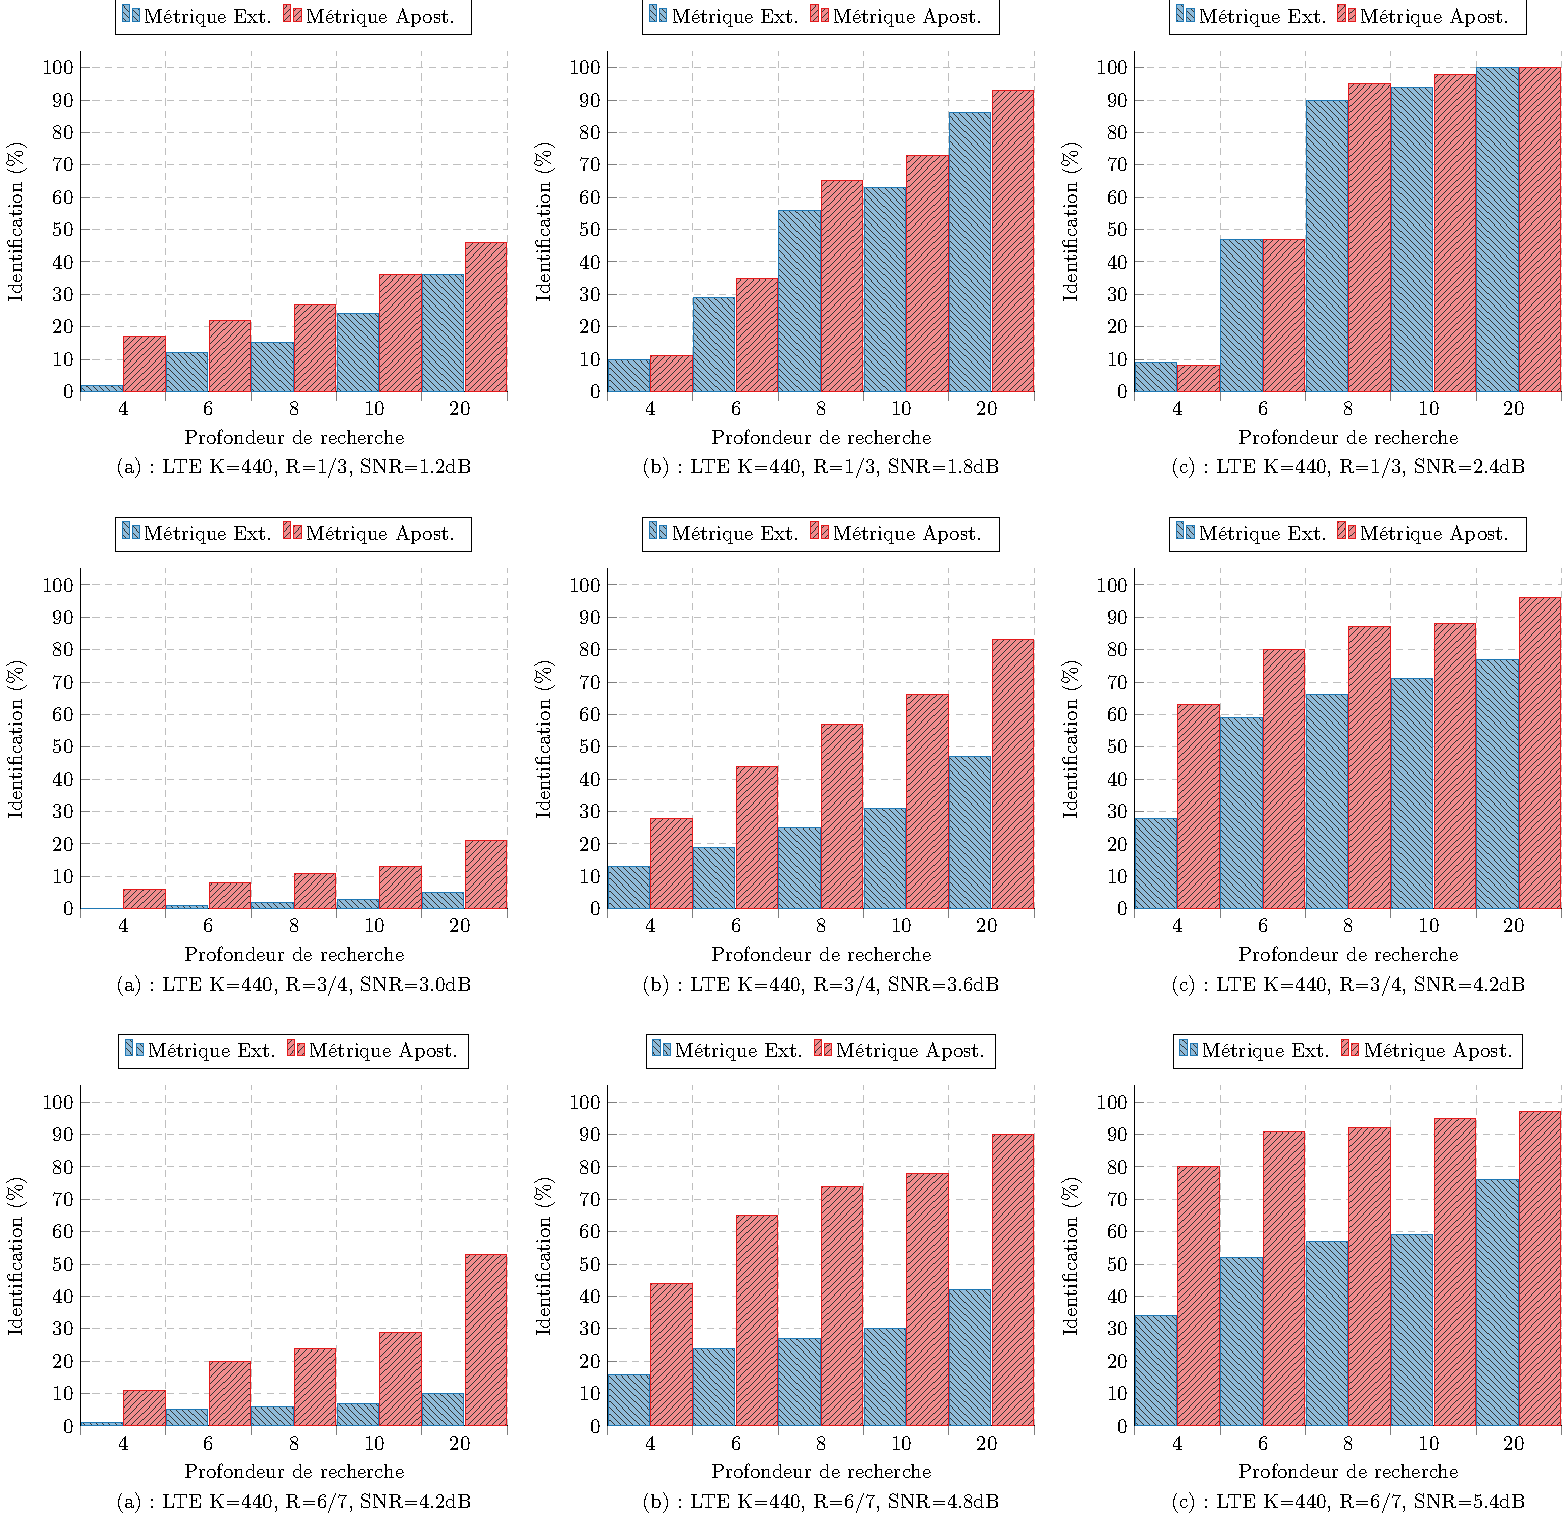
\includegraphics[width=1.05\textwidth]{main/ch3_fig/id2/dvb/tikz/440.pdf}
	\caption{Pourcentage d'identification pour différents turbo codes du standard DVB-RCS K=440, R=1/3, 3/4 et 6/7.
	Décodage EML-MAP itérant 8 fois. \label{fig:dvb440}}
\end{figure}

\begin{figure}[!t]
	\centering
	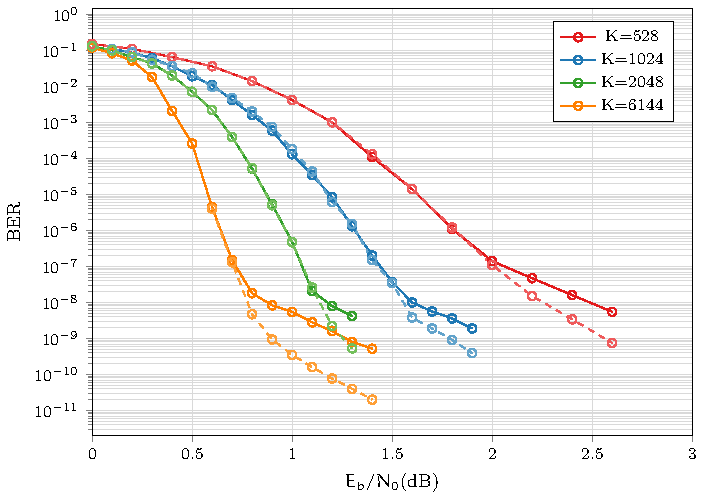
\includegraphics[width=\textwidth]{main/ch3_fig/fnc/lte/tikz/lte_ber.pdf}
	\caption{Comparaison de performances de décodages en terme de taux d'erreur binaire entre EML-MAP et FNC. Standard LTE, K=528, 1024, 2048 et 6144. R=1/3.
	Décodeurs itérant jusqu'à 8 fois. \label{fig:fnc_lte_ber}}
\end{figure}

% \begin{figure}[!t]
% 	\centering
% 	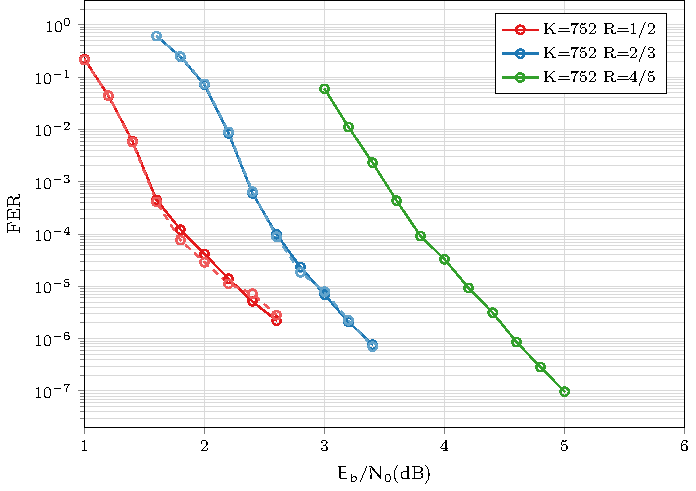
\includegraphics[width=\textwidth, draft]{main/ch3_fig/fnc/dvb/tikz/dvb1_752.pdf}
% 	\caption{Comparaison de performances de décodages entre EML-MAP et FNC. Standard DVB-RCS, K=752. R=1/3, 1/2, 3/4 et 6/7.
% 	Décodeurs itérant jusqu'à 8 fois. \label{fig:fnc_dvb_752}}
% \end{figure}

\begin{figure}[!t]
\centering
			%!TEX root = ../../../my_thesis.tex
\begin{tikzpicture}
	\begin{semilogyaxis}[footnotesize, width=0.9\linewidth, height=0.6\linewidth,    
			xmin=0, xmax=3, xtick={0,0.4,...,3.0},
			ymin=1e-7,  ymax=1,
			xlabel=$E_b/N_0 \text{(dB)}$, ylabel=FER,  grid=both, grid style={gray!30},
		tick align=outside, tickpos=left, legend pos=north east]
																				
	%	\addplot[mark=o,Paired-1]  table [x=SNR, y=FER] {main/ch1_fig/std/lte13_528.dat}; 
	%	\addplot[mark=diamond,Paired-3]  table [x=SNR, y=FER] {main/ch1_fig/std/lte13_1504.dat}; 
	%	\addplot[mark=square,Paired-5]  table [x=SNR, y=FER] {main/ch1_fig/std/lte13_2048.dat}; 
	%	\addplot[mark=triangle,Paired-7]  table [x=SNR, y=FER2] {main/ch1_fig/std/lte13_6144.dat}; 
																						
																														
	%	\legend{K=528, K=1504, K=2048, K=6144}

	\node[Paired-5,above,rotate=30] at (axis cs:1.5,10e-4){\Huge Simulations en cours};																														
	\end{semilogyaxis}
\end{tikzpicture}  	
	\caption{Comparaison de performances de décodages entre EML-MAP et FNC. Standard DVB-RCS, K=752. R=1/3, 1/2, 3/4 et 6/7.
	Décodeurs itérant jusqu'à 8 fois. \label{fig:fnc_dvb_752}}
\end{figure}